% fig_arch.tex - CollaRAG overall architecture (standalone -> PDF)
\documentclass[tikz,border=6pt]{standalone}
\usepackage{tikz}
\usetikzlibrary{arrows.meta,positioning,fit,backgrounds,calc,shapes.geometric}
\definecolor{ours}{HTML}{C0392B}
\definecolor{slate}{HTML}{2C3E50}
\definecolor{teal}{HTML}{16A085}
\definecolor{purp}{HTML}{8E44AD}
\definecolor{blue}{HTML}{2980B9}
\definecolor{lg}{HTML}{ECF0F1}
\definecolor{mg}{HTML}{BDC3C7}
\definecolor{mgd}{HTML}{7F8C8D}
\begin{document}
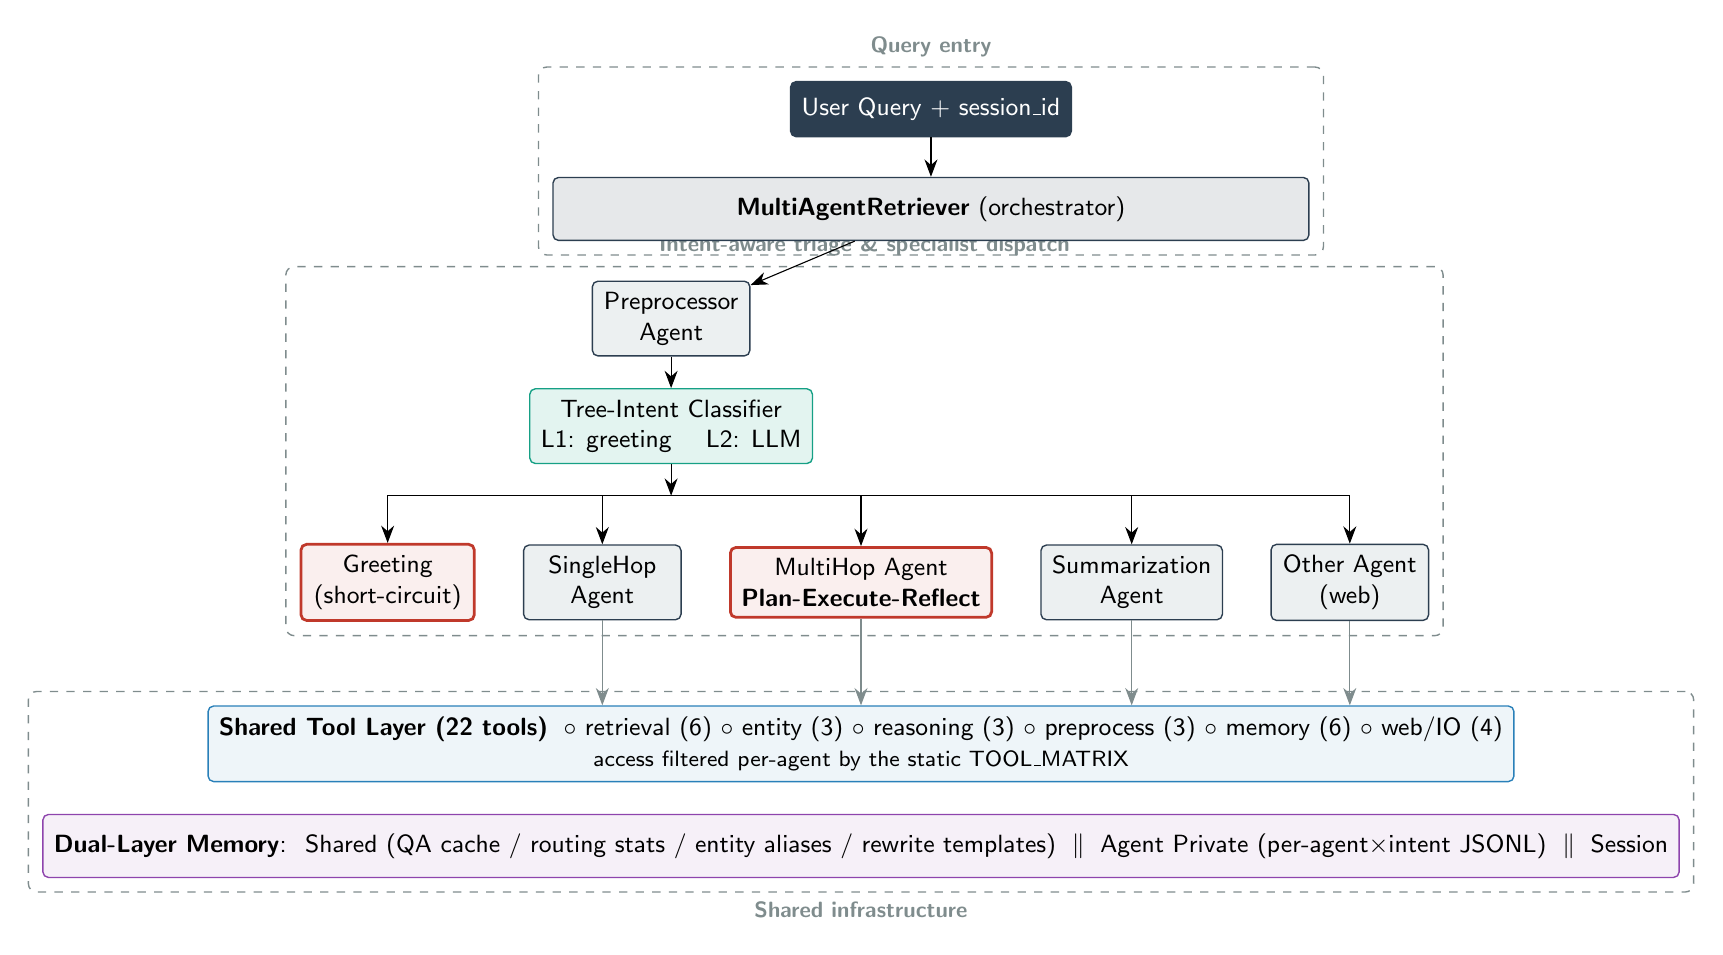
\begin{tikzpicture}[
  font=\small\sffamily,
  >={Stealth[length=2.2mm]},
  node distance=4mm and 6mm,
  box/.style={draw=slate, rounded corners=2pt, align=center, inner sep=4pt,
              minimum height=7mm, fill=white, line width=0.5pt},
  agent/.style={box, fill=lg, minimum width=20mm, minimum height=8mm},
  ours/.style={box, draw=ours, line width=1pt, fill=ours!8, minimum width=22mm, minimum height=8mm},
  hub/.style={box, fill=slate!12, minimum width=30mm, minimum height=8mm},
  layer/.style={draw=mgd, dashed, rounded corners=3pt, inner sep=5pt, line width=0.5pt},
  cat/.style={font=\footnotesize\sffamily\bfseries, color=mgd},
]
% --- user query ---
\node[box, fill=slate, text=white, minimum width=34mm] (q) {User Query + session\_id};

% --- orchestrator container ---
\node[hub, below=5mm of q, minimum width=96mm] (orch) {\textbf{MultiAgentRetriever} (orchestrator)};

% --- preprocessor ---
\node[agent, below=5mm of orch.south, xshift=-33mm] (pre) {Preprocessor\\Agent};

% --- classifier ---
\node[hub, below=of pre, minimum width=34mm, fill=teal!12, draw=teal] (cls)
  {Tree-Intent Classifier\\L1: greeting \quad L2: LLM};

% --- five specialists ---
\node[ours, below=10mm of cls.south, xshift=-36mm] (g) {Greeting\\(short-circuit)};
\node[agent, right=of g] (sh) {SingleHop\\Agent};
\node[ours, right=of sh] (mh) {MultiHop Agent\\\textbf{Plan-Execute-Reflect}};
\node[agent, right=of mh] (sm) {Summarization\\Agent};
\node[agent, right=of sm] (ot) {Other Agent\\(web)};

% --- shared tool layer ---
\node[box, fill=blue!8, draw=blue, below=11mm of mh.south, minimum width=104mm,
      minimum height=9mm, align=center] (tools)
  {\textbf{Shared Tool Layer (22 tools)} $\;\circ$ retrieval (6) $\circ$ entity (3) $\circ$ reasoning (3) $\circ$ preprocess (3) $\circ$ memory (6) $\circ$ web/IO (4)\\
   \footnotesize access filtered per-agent by the static TOOL\_MATRIX};

% --- dual-layer memory ---
\node[box, fill=purp!8, draw=purp, below=4mm of tools.south, minimum width=104mm,
      minimum height=8mm, align=center] (mem)
  {\textbf{Dual-Layer Memory}: \;Shared (QA cache / routing stats / entity aliases / rewrite templates)
   \;$\Vert$\; Agent Private (per-agent$\times$intent JSONL) \;$\Vert$\; Session};

% --- edges ---
\draw[->] (q) -- (orch);
\draw[->] (orch) -- (pre);
\draw[->] (pre) -- (cls);
\coordinate (junc) at ($(cls.south)+(0,-4mm)$);
\draw[->] (cls.south) -- (junc);
\draw[->] (junc) -| (g.north);
\draw[->] (junc) -| (sh.north);
\draw[->] (junc) -| (mh.north);
\draw[->] (junc) -| (sm.north);
\draw[->] (junc) -| (ot.north);

\foreach \n in {sh,mh,sm,ot} \draw[->, mgd] (\n.south) -- (\n.south |- tools.north);

\begin{scope}[on background layer]
  \node[layer, fit=(q)(orch), label={[cat]above:Query entry}] {};
  \node[layer, fit=(pre)(cls)(g)(sh)(mh)(sm)(ot), label={[cat]above:Intent-aware triage \& specialist dispatch}] {};
  \node[layer, fit=(tools)(mem), label={[cat]below:Shared infrastructure}] {};
\end{scope}
\end{tikzpicture}
\end{document}
